\subsection{标注}
\subsubsection{string 类型}
可包括各种符号,用双引号 " 或单引号 ' 包括起来。空格和换行都会保持不变。
当遇到引号或其他特殊符号时,用\ref{markcode}所示格式进行转义变换。
\begin{table}[htb]
\rowcolors{1}{white}{whiteblue}
\centering
 \caption{ string 类型对应的特殊字符}\label{markcode}
 \begin{tabular}{cc|cc}
  \toprule
    \textbf{换码序列} & \textbf{对应的字符} & \textbf{换码序列} &
    \textbf{对应的字符}\\\midrule
    \verb|\'| & 单引号~\verb|'| & \verb|\"| & 双引号~\verb|"| \\
    \verb|\?| & \verb|?| & \verb|\\| & \verb|\| \\
    \verb|\a| & 报警 & \verb|b| & 退格 \\
    \verb|\f| & 进纸 & \verb|\n| & 换行 \\
    \verb|\r| & 回车 & \verb|\t| & 水平制表符 \\
    \verb|\v| & 竖直制表符 & & \\
    \verb|\0|--\verb|\377| & 八进制编码相应的字符 &
    \verb|\x0|--\verb|\xFF| & 十六进制编码相应的字符 \\
  \bottomrule
 \end{tabular}

\end{table}

\subsubsection{点上的标注}
调用代码如下:

\begin{asycmd}
label(Label,position,align);\\
label("字符串", 点);\\
label("字符串", 点, 方向);\\
Label("字符串",字符旋转方向);\\
label(Label("字符串",字符旋转方向),点,相对点方向);
\end{asycmd}
label 的相对点方向方向有东南西北左中右\textcolor[rgb]{0.00,0.50,0.25}{ LeftSide,RightSide,Center 和 Relative(E或(S,N,W))}\\
Label 的字符旋转方向有东南西北任意角度 \textcolor[rgb]{0.00,0.50,0.25}{Rotate(E或(S,N,W))或 Rotate(x,y)}\\

  \lstinputlisting{body/asycode/label.asy}

\begin{figure}[htbp]
  % Requires \usepackage{graphicx}
  \centering
  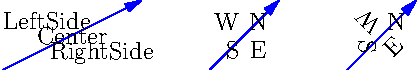
\includegraphics[width=14cm]{body/asycode/label}\\
  \caption{标注方向}\label{label}
\end{figure}


\subsubsection{坐标轴标注}

\begin{lstlisting}
xaxis("$x$",Arrow); //`X 轴下方`
yaxis("$y$",Arrow);//`Y 轴左方` 
\end{lstlisting}



\subsubsection{箭头标注}
\color{red}
\verb|arrow("$t=\frac{1}{3}$",Z,SE);|
\normalcolor

Z 为 pair 类型的点,SE 为相对方向,引号内为标注文字

\subsubsection{中文标注}

在含有中文字符时,前面须加上以下命令:
\begin{lstlisting}
texpreamble("\usepackage{CJK}
 \AtBeginDocument{\begin{CJK*}{GBK}{kai}
   \AtEndDocument{\clearpage\end{CJK*}}");}
\end{lstlisting}

\clearpage
